\chapter{Results}
\label{chapter:results}

Combining all the methods and algorithms from the previous chapters, such as\\ approximation, clustering and outlier detection, gives us insight into the \Calcium concentration data. We give an algorithm for detecting activated t cells, look at differences between mouse and human t cells, analyse the oscillations and investigate whether there are different types of activated t cells.

\section{Proposed Algorithm for Detecting Activated T Cells}
\label{sec:proposed-algorithm}

A relevant question this work aims to provide an answer to is, how pre-activated,\\ unactivated and activated t cells can be distinguished.

First we give a method for filtering the pre-activated cells from a dataset. From their nature we expect a high value in \Calcium concentration at the start of the recording. Using the approximation from chapter~\ref{chapter:approximating} it is easy to get the approximate \Calcium concentration value at the start of the recording, as it is the parameter $u$. Using the algorithm~\ref{alg:outlier_detection} with parameters threshold as $[\infty, 0.5]$ and parameters\_used as [$u$] gives good results. It returns the indices of particles, which are pre-activated in the data sets of the positive controls.

After having filtered out pre-activated particles, we want to distinguish between\\ unactivated and activated particles. For this we propose the following steps:

\begin{enumerate}
	\item get positive control, negative control and experiment recordings
	\item transform each particle time series of all three data sets to the parameter list by approximating it with a combination of sigmoid functions, according to chapter~\ref{chapter:approximating}, using the algorithm \ref{alg:main}
	\item normalise each of the parameters of all data sets, such that the mean is 0 and the standard deviation is 1
	\item use outlier detection, which is described in algorithm~\ref{alg:outlier_detection}, to filter out non-conforming cells from both the positive and negative control, as well as pre-activated cells, and particles where the approximation yielded suboptimal results
	\item sample particles from the filtered positive and negative control groups to match the number of particles in the both groups
	\item use clustering method, as one of the two described in chapter~\ref{chapter:clustering}, with parameters of selected negative and positive control as input to get the clustering parameters
	\item predict the membership of the experiment particle parameters to the clusters to get a prediction of activation
\end{enumerate}

The third and fifth step is beneficial when clustering, as many clustering methods expect equally sized clusters that are centred and have equal standard deviation. 

This algorithm is implemented in Python and shown in appendix~\ref{chapter:python_implementation}. Applying this to a positive, negative control and an experiment data sets of mouse t cells gives the exemplary results shown in table~\ref{tab:results_main_algorithm}. The experiment dataset contains t cells that came in contact with a medium density of MHC-peptide complex replicas. The number of activated cells detected in the positive and negative control are shown as a reference point. Comparing them in the case illustrated suggests that in this case Gaussian Mixture Model is the better clustering algorithm.

\begin{table}[h]
	\centering
	\begin{tabular}{|c|c|c|c|c|}
		\hline
		 & file & activated & out of & percentage\\
		 \hline
		  & negative control & 47 & 969 & 4.850\%\\
		 gaussian mixture & positive control & 932 & 969 & 96.182\%\\
		  & experiment & 716 & 890 & 80.449\%\\
		 \hline
		  & negative control & 53 & 969 & 5.470\%\\
		 k-means & positive control & 926 & 969 & 95.562\%\\
		  & experiment & 687 & 890 & 77.191\%\\
		 \hline
	\end{tabular}
	\caption{Output of the proposed algorithm applied to three files of mouse t cells.}
	\label{tab:results_main_algorithm}
\end{table}

The algorithm can be adapted by using different clustering methods, or specifying other methods of separating the particles based on the parameters derived.

\section{Difference between Mouse and Human Cells}
\label{sec:differences_between_mouse_and_human_cells}

Now, that we have an algorithm for detecting activated cells, we might ask whether there are notable differences between mouse and human cells. Plotting all data points in a single plot, as seen in figure~\ref{fig:all_cells}, shows whether differences are to be expected.

\begin{figure}[h]
	\centering
	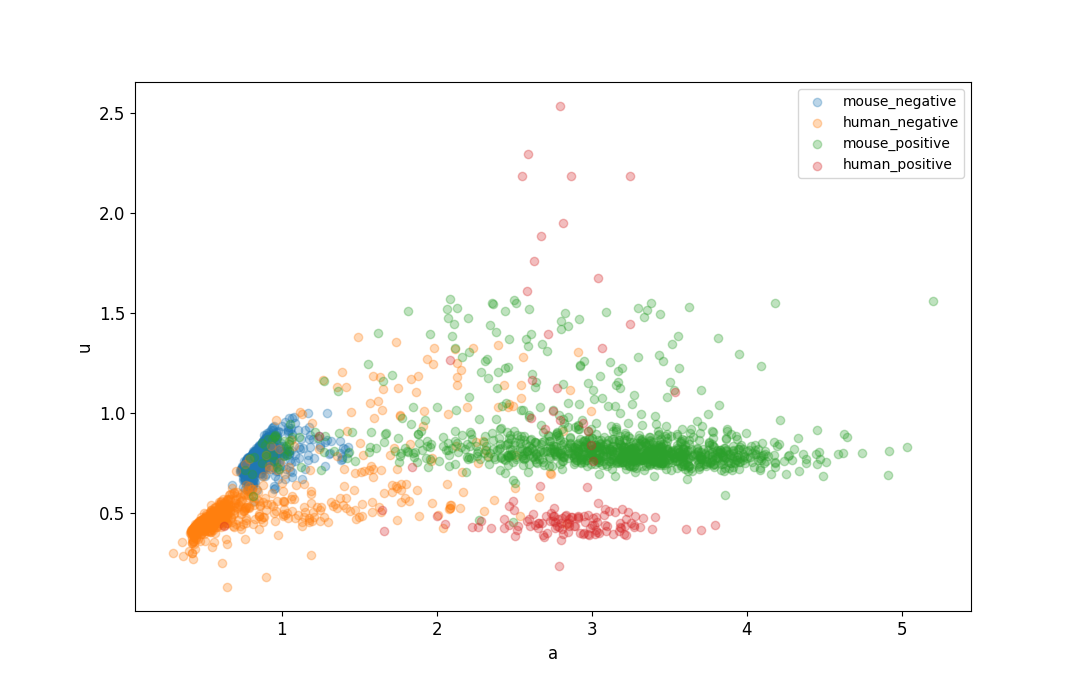
\includegraphics[width=\textwidth]{fig/all_cells}
	
	\caption{All data points from the four control data sets plotted along the axes activated value $a$ and unactivated values $u$.}
	\label{fig:all_cells}
\end{figure}

Differences in the axes $a$ and $u$ are present. On average the unactivated value $u$ and activated value $a$ are bigger in mouse t cells than the human counterparts. Looking at each of the parameters gathered from the approximation is possible by using the means and standard deviation of each parameter. These values are displayed in table~\ref{tab:mean_std_parameters}. It shows the mean $\mu$ and standard deviation $\sigma$ of the negative and positive control of mouse and human t cells.

\begin{table}[h!]
	\centering
	\begin{tabular}{|c|c|c|c|c|c|c|c|c|c|}
		\hline
		& & & $a$ & $u$ & $d$ & $k1$ & $k2$ & $w1$ & $w2$\\
		\hline
		\multirow{4}{*}{\rotatebox[origin=c]{90}{mouse}} & \multirow{2}{*}{\rotatebox[origin=c]{90}{pos}} & $\mu$ & 3.083 & 0.85 & 1.698 & 0.08 & -0.052 & 300.77 & 491.275\\
		\cline{3-10}
		& & $\sigma$ & 0.72 & 0.159 & 0.33 & 0.085 & 0.07 & 82.451 & 104.304\\
		\cline{2-10}
		& \multirow{2}{*}{\rotatebox[origin=c]{90}{neg}} & $\mu$ & 0.862 & 0.77 & 0.788 & 1.262 & -0.075 & 88.644 & 304.531\\
		\cline{3-10}
		& & $\sigma$ & 0.106 & 0.057 & 0.053 & 1.219 & 0.148 & 99.833 & 184.08\\
		\hline
		\multirow{4}{*}{\rotatebox[origin=c]{90}{human}} & \multirow{2}{*}{\rotatebox[origin=c]{90}{pos}} & $\mu$ & 2.854 & 0.553 &  1.916 & 0.23 & -0.033 & 113.595 & 438.763\\
		\cline{3-10}
		& & $\sigma$ & 0.357 & 0.294 & 0.44 & 0.219 & 0.073 & 59.7 & 175.998\\
		\cline{2-10}
		& \multirow{2}{*}{\rotatebox[origin=c]{90}{neg}} & $\mu$ & 0.864 & 0.543 & 0.604 & 0.58 & -0.19 & 169.394 & 528.006 \\
		\cline{3-10}
		& & $\sigma$ & 0.56 & 0.197 & 0.274 & 1.022 & 0.332 & 142.358 & 229.078 \\
		\hline
	\end{tabular}
	\caption{Mean $\mu$ and standard deviation $\sigma$ of the parameters of the approximation for positive and negative controls in human and mouse cells.}
	\label{tab:mean_std_parameters}
\end{table}

By comparing the means from table~\ref{tab:mean_std_parameters} we see that indeed the mean of $a$ and $u$ are higher or about equal in mouse cells. Differences in $d$, $k1$ and $k2$ are less pronounced and differ between positive and negative control. Differences in $w1$ and $w2$ are probably caused by differences in timing between the different recordings of the control groups. Therefore, comparing the means does not give much valuable information. In conclusion the differences are biggest in the parameter $u$.

\newpage
\section{Oscillation in Decrease}
\label{sec:oscillation_in_decrease}

Looking at the frequencies, amplitudes and phases returned from the approximation\\ described in section~\ref{sec:adding_oscillation_to_the_approximation} gives us an idea with which period the typical t cell oscillates in \Calcium concentration during the decrease after activation. The figure~\ref{fig:freq_amp} shows violin plots of all three parameters in the positive control on human t cells. The means in this data set are 0.005 for the frequency, 0.01 for the amplitude and -0.001 for the phase. The details of the density distribution are shown in the width of each of the violin plots.

As some t cells do not oscillate, the approximation sometimes returns a misleading\\ frequency with a low amplitude. We want to filter these cells before looking at the typical period with which the \Calcium concentration oscillates. We choose arbitrary threshold values, that seemed sensible to the author. Namely, all particles with an amplitude less than 0.1 or a frequency less than 0.005 are removed before once again looking at the average values. Now the average frequency is 0.008 with an average amplitude of 0.223. This corresponds to a period of oscillation being $1/freq = $ 125 seconds. Indeed, looking at the example provided in figure~\ref{fig:freq_amp}, this seems like a good estimate.

Lastly we compare this to the positive control in mouse cells. Before filtering the averages are 0.007 for the frequency, 0.071 for the amplitude and 0.288 for the phase. After filtering, with the same thresholds as for human cells, we have an average of 0.007 for the frequency and 0.177 for the amplitude. Converting this to the period gives us 143 seconds. This compares to the average period found in human t cells.

\begin{figure}[h!]
	\centering
	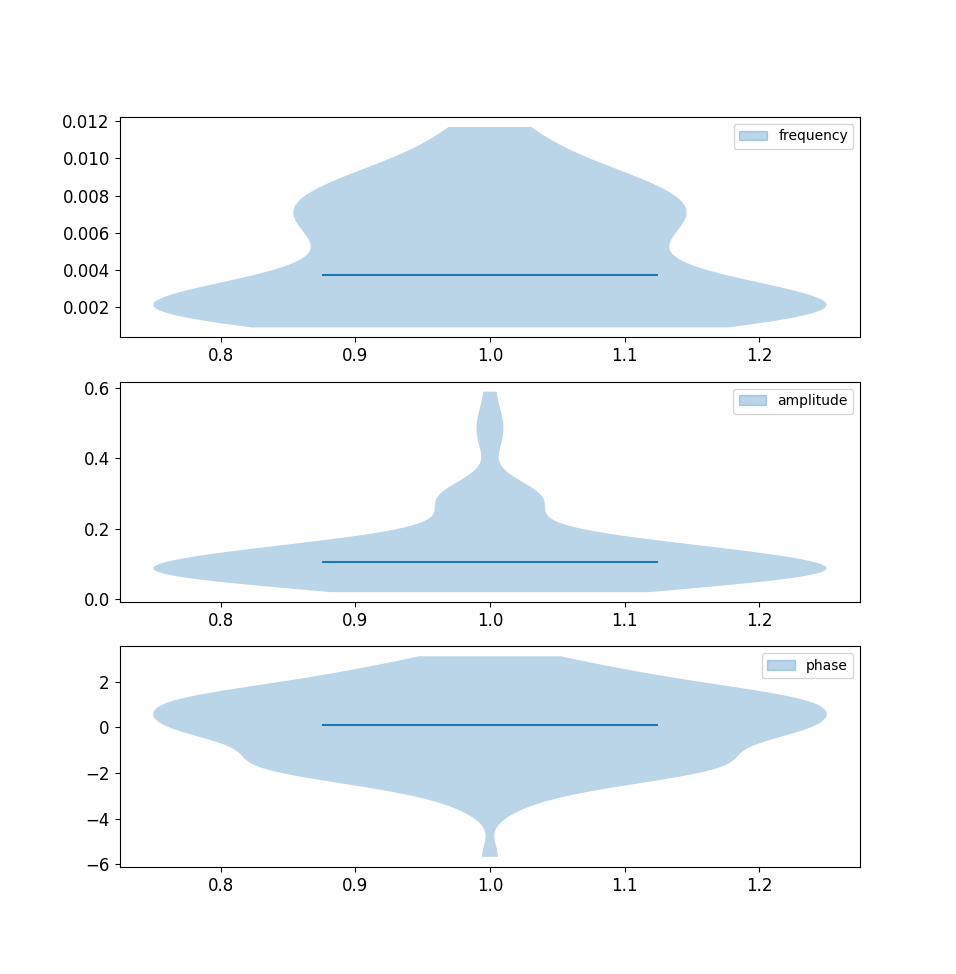
\includegraphics[width=0.9\textwidth]{fig/freq_amp}
	
	\caption{Violin plots of the frequencies, amplitudes and phases of the oscillation\\ approximation in the positive control dataset of human t cells.}
	\label{fig:freq_amp}
\end{figure}

\newpage
\section{Types of Activated Cells}

It is interesting to see whether there are different types of activated cells. We find an answer by looking at the activated cells only. We have two data sets of activated cells, one from mouse cells and one from human cells. Naturally there will be differences between the two. This was further explored in section~\ref{sec:differences_between_mouse_and_human_cells}. By looking at only one data set of the positive control at a time we generate the images seen in figure~\ref{fig:positive_control}. To reduce the dimensionality once again Principal Component Analysis is used.

From figure~\ref{fig:positive_control}, it is not apparent that there are different types of activated cells.

Lastly we can have a look whether particles differ in the oscillation. Using the\\ approximation of the oscillation and the filtering done in section~\ref{sec:oscillation_in_decrease} we can for example differ between oscillating t cells, marked by high amplitude and period around the expected 125 seconds, and non-oscillating t cells, marked by low amplitude or different period.

We note that out of 139 particles in the positive control of human t cells only 14 have the behaviour of a heavily oscillating t cell. In the mouse positive control it is 192 out of 1058.

\begin{figure}[h]
	\centering
	\begin{subfigure}{0.49\linewidth}
		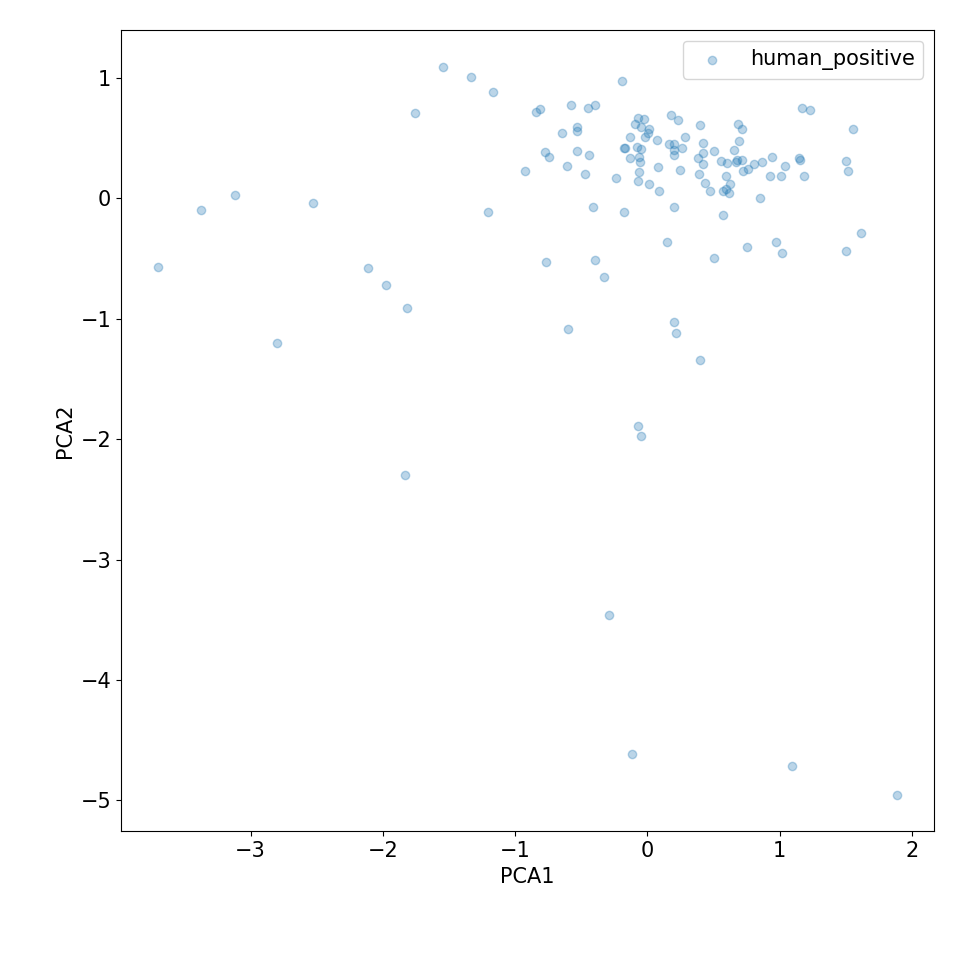
\includegraphics[width=\textwidth]{fig/positive_control_human}
	\end{subfigure}
	\hfill
	\begin{subfigure}{0.49\linewidth}
		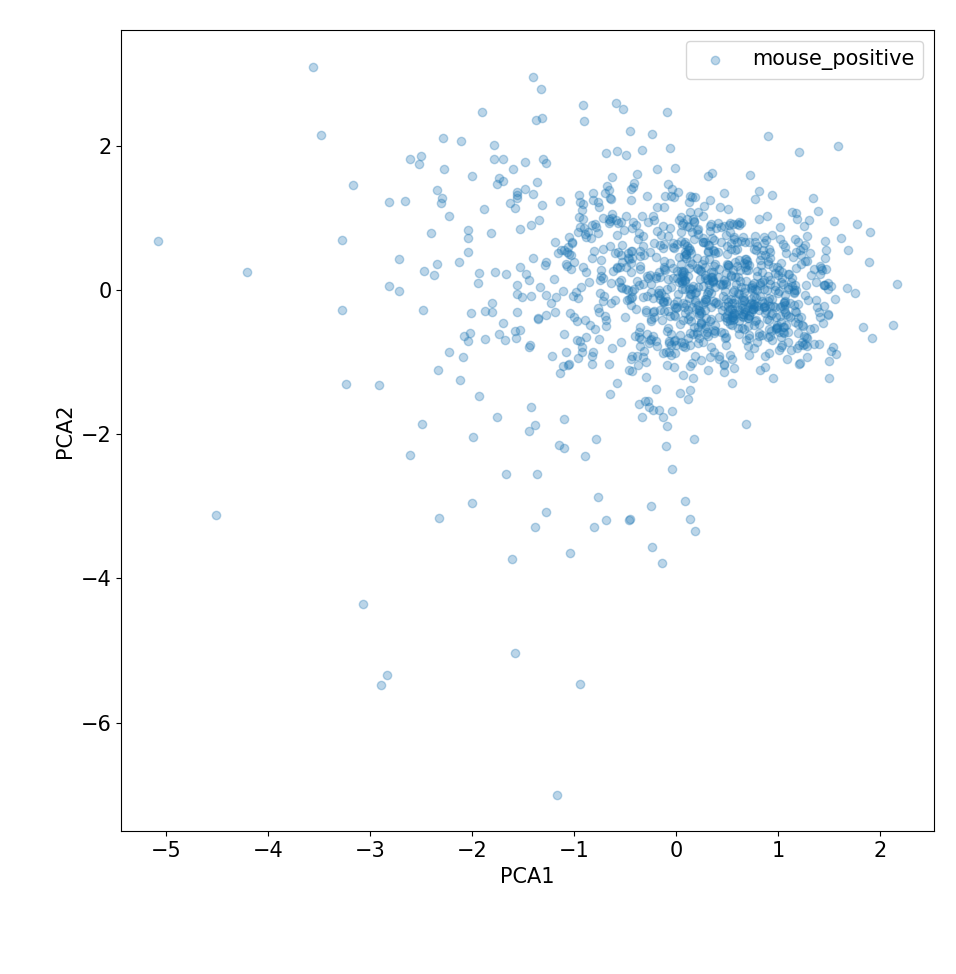
\includegraphics[width=\textwidth]{fig/positive_control_mouse}
	\end{subfigure}
	
	\caption{First two axes of the Principal Component Analysis of activated human and mouse t cells. There appear not be any major differences between the two types of t cells.}
	\label{fig:positive_control}
\end{figure}